\chapter{Day 1 Overview}
\label{ch-day1}


% ******************************************************************
% ******************************************************************
% ******************************************************************
\clearpage
\newpage
\section{Nuclear Power Plant with 3D motions from SW4}
\label{Nuclear_Power_Plant_with_3D_motions_from_SW4}

The Real-ESSI input files for this example are available 
\href{https://github.com/yuan-energy/Real-ESSI-Short-Course-Examples/tree/master/short-course-examples/Day1/Nuclear_Power_Plant_with_3D_motions_from_SW4}{HERE}. 
The compressed package of Real-ESSI input files for this example is available 
\href{https://github.com/yuan-energy/Real-ESSI-Short-Course-Examples/blob/master/short-course-examples/Day1/Nuclear_Power_Plant_with_3D_motions_from_SW4/Nuclear_Power_Plant_with_3D_motions_from_SW4.tgz?raw=true}{HERE}. 

\begin{figure}[H]
  \centering
  \includegraphics[width = 9cm]{./Figure-files/Day1/Nuclear_Power_Plant_with_3D_motions_from_SW4/overview.png}
  \caption{Simulation Model}
  \label{fig_NPP_3D_overview_3D_motion}
\end{figure}

The Modeling parameters are listed.
\begin{itemize}
  \item Soil 
  \begin{itemize}
    \item Unit weight, $\gamma$, \enspace \enspace 21.4 kPa
    \item Shear velocity, $Vs$, \enspace \enspace 500 m/s
    \item Young's modulus, $E$, \enspace \enspace 1.3 GPa
    \item Poisson's ratio, $\nu$, \enspace \enspace 0.25
    \item Shear strength, $S_u$, \enspace \enspace 650 kPa
    \item von Mises radius, $k$, \enspace \enspace 60 kPa
    \item kinematic hardening, $H_a$, \enspace \enspace 30 MPa
    \item kinematic hardening, $C_r$, \enspace \enspace 25
  \end{itemize}
  \item Structure
  \begin{itemize}
    \item Unit weight, $\gamma$, \enspace \enspace 24 kPa
    \item Young's modulus, $E$, \enspace \enspace 20 GPa
    \item Poisson's ratio, $\nu$, \enspace \enspace 0.21
  \end{itemize}
\end{itemize}

The input motion at the bottom is a 3D wave from SW4.

SIMULATION TIME: With 32 cores on AWS EC2 c4.8xlarge instance, the running time for this example is 17 hours.

% ******************************************************************
% ******************************************************************
% ******************************************************************
\clearpage
\newpage
\section{Nuclear Power Plant with 1D motions from Deconvolution}
\label{Nuclear_Power_Plant_with_1D_motions_from_Deconvolution}

The Real-ESSI input files for this example are available 
\href{https://github.com/yuan-energy/Real-ESSI-Short-Course-Examples/tree/master/short-course-examples/Day1/Nuclear_Power_Plant_with_1D_motions_from_Deconvolution}{HERE}. 
The compressed package of Real-ESSI input files for this example is available 
\href{https://github.com/yuan-energy/Real-ESSI-Short-Course-Examples/blob/master/short-course-examples/Day1/Nuclear_Power_Plant_with_1D_motions_from_Deconvolution/Nuclear_Power_Plant_with_1D_motions_from_Deconvolution.tgz?raw=true}{HERE}. 

\begin{figure}[H]
  \centering
  \includegraphics[width = 7cm]{./Figure-files/Day1/Nuclear_Power_Plant_with_1D_motions_from_Deconvolution/overview.png}
  \caption{Simulation Model}
  \label{fig_NPP_3D_overview_1D_motion}
\end{figure}

The input motion at the bottom is the deconvolution of the Northridge earthquake records. 

\begin{figure}[H]
  \centering
  \includegraphics[width = 7cm]{./Figure-files/Day1/Nuclear_Power_Plant_with_1D_motions_from_Deconvolution/scaled_NORTHR_x_A.jpg}
  \includegraphics[width = 7cm]{./Figure-files/Day1/Nuclear_Power_Plant_with_1D_motions_from_Deconvolution/scaled_NORTHR_x_D.jpg}
  \caption{Motion Deconvolution}
  \label{fig_motion_deconvolution1}
\end{figure}

The Modeling parameters are listed.
\begin{itemize}
  \item Soil 
  \begin{itemize}
    \item Unit weight, $\gamma$, \enspace \enspace 21.4 kPa
    \item Shear velocity, $Vs$, \enspace \enspace 500 m/s
    \item Young's modulus, $E$, \enspace \enspace 1.3 GPa
    \item Poisson's ratio, $\nu$, \enspace \enspace 0.25
    \item Shear strength, $S_u$, \enspace \enspace 650 kPa
    \item von Mises radius, $k$, \enspace \enspace 60 kPa
    \item kinematic hardening, $H_a$, \enspace \enspace 30 MPa
    \item kinematic hardening, $C_r$, \enspace \enspace 25
  \end{itemize}
  \item Structure
  \begin{itemize}
    \item Unit weight, $\gamma$, \enspace \enspace 24 kPa
    \item Young's modulus, $E$, \enspace \enspace 20 GPa
    \item Poisson's ratio, $\nu$, \enspace \enspace 0.21
  \end{itemize}
\end{itemize}

% ******************************************************************
% ******************************************************************
% ******************************************************************
\clearpage
\newpage
\section{Nuclear Power Plant with 3$\times$1D motions from Deconvolution}
\label{Nuclear_Power_Plant_with_3by1D_motions_from_Deconvolution}

The Real-ESSI input files for this example are available 
\href{https://github.com/yuan-energy/Real-ESSI-Short-Course-Examples/tree/master/short-course-examples/Day1/Nuclear_Power_Plant_with_3by1D_motions_from_Deconvolution}{HERE}. 
The compressed package of Real-ESSI input files for this example is available 
\href{https://github.com/yuan-energy/Real-ESSI-Short-Course-Examples/blob/master/short-course-examples/Day1/Nuclear_Power_Plant_with_3by1D_motions_from_Deconvolution/Nuclear_Power_Plant_with_3by1D_motions_from_Deconvolution.tgz?raw=true}{HERE}. 

\begin{figure}[H]
  \centering
  \includegraphics[width = 9cm]{./Figure-files/Day1/Nuclear_Power_Plant_with_3by1D_motions_from_Deconvolution/overview.png}
  \caption{Simulation Model}
  \label{fig_NPP_3D_overview_3by1Dmotion}
\end{figure}


The input motion at the bottom is the deconvolution of the Northridge earthquake records. 

\begin{figure}[H]
  \centering
  \includegraphics[width = 5cm]{./Figure-files/Day1/Nuclear_Power_Plant_with_3by1D_motions_from_Deconvolution/scaled_NORTHR_x_A.jpg}
  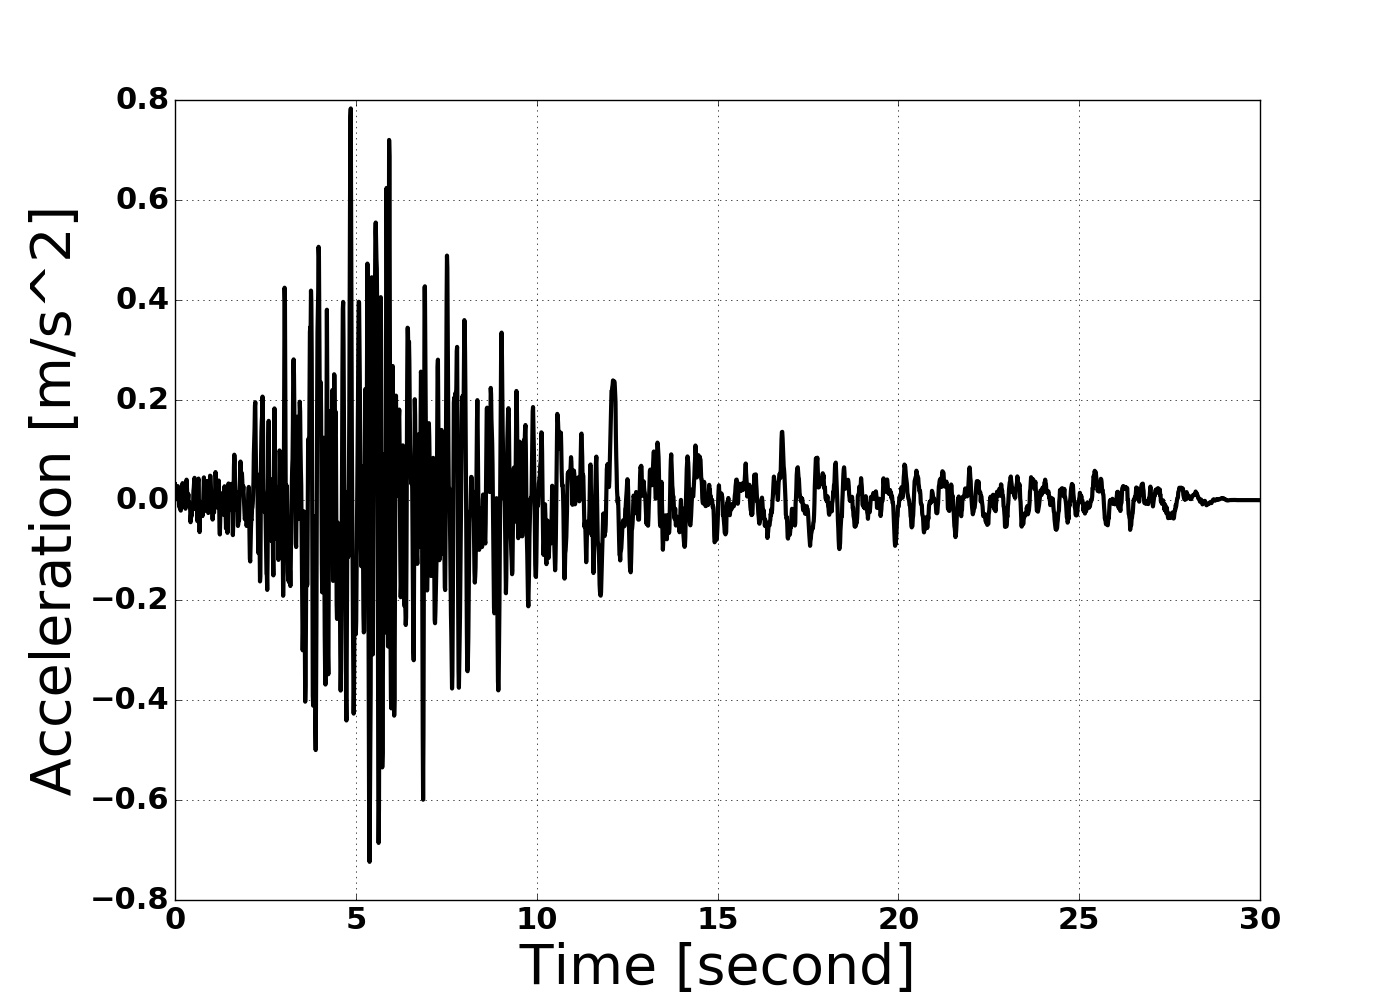
\includegraphics[width = 5cm]{./Figure-files/Day1/Nuclear_Power_Plant_with_3by1D_motions_from_Deconvolution/scaled_NORTHR_y_A.jpg}
  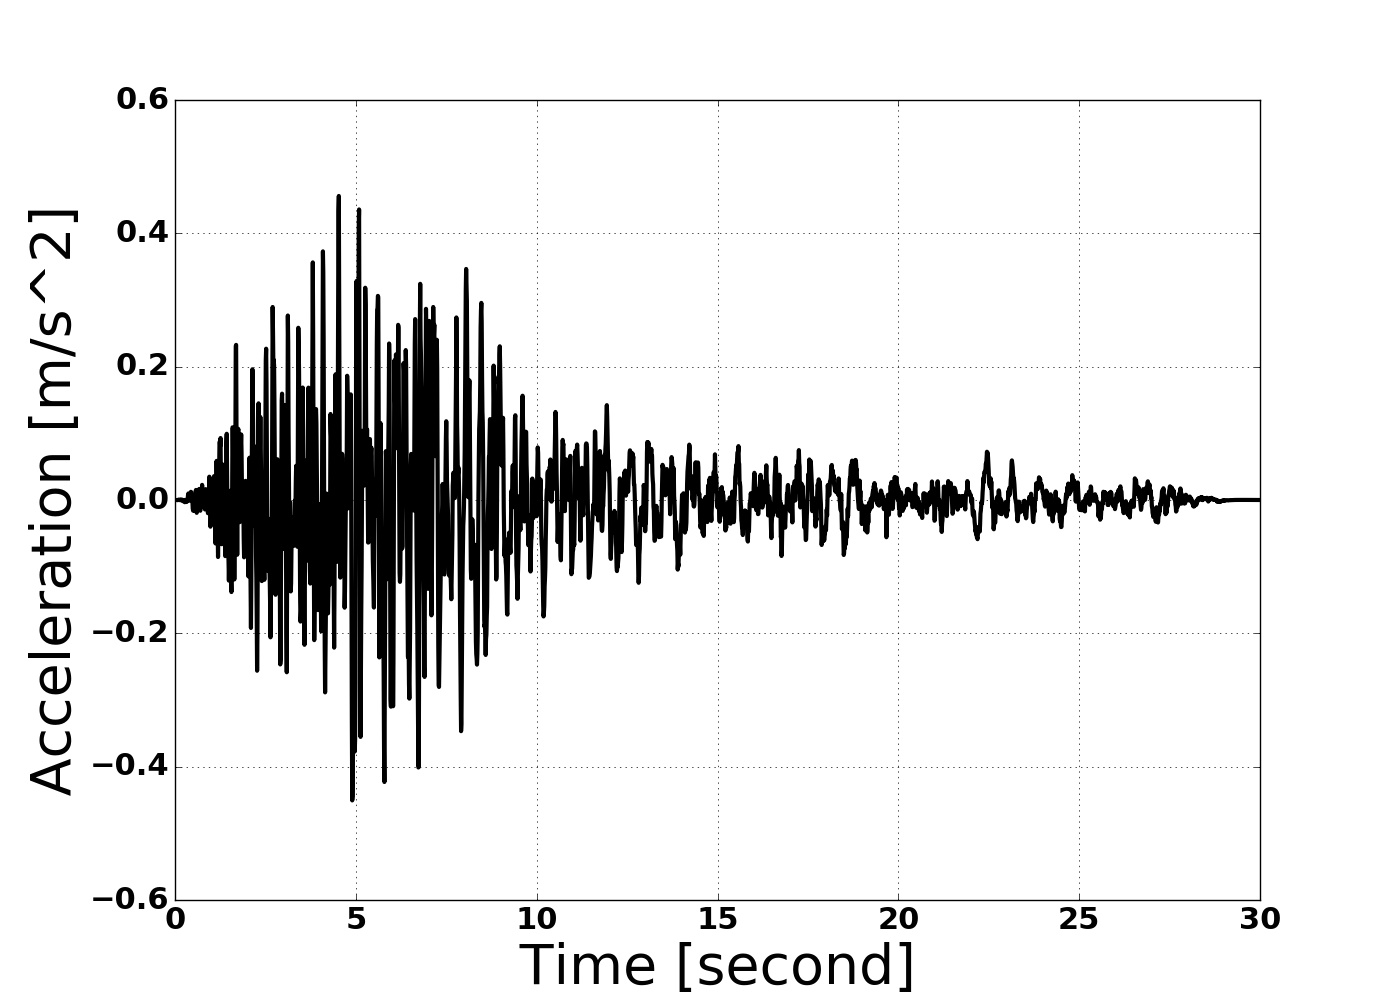
\includegraphics[width = 5cm]{./Figure-files/Day1/Nuclear_Power_Plant_with_3by1D_motions_from_Deconvolution/scaled_NORTHR_z_A.jpg}
  \caption{Acceleration Deconvolution, from left to right in x, y, z directions respectively. }
  \label{fig_motion_deconvolution2}
\end{figure}

\begin{figure}[H]
  \centering
  \includegraphics[width = 5cm]{./Figure-files/Day1/Nuclear_Power_Plant_with_3by1D_motions_from_Deconvolution/scaled_NORTHR_x_D.jpg}
  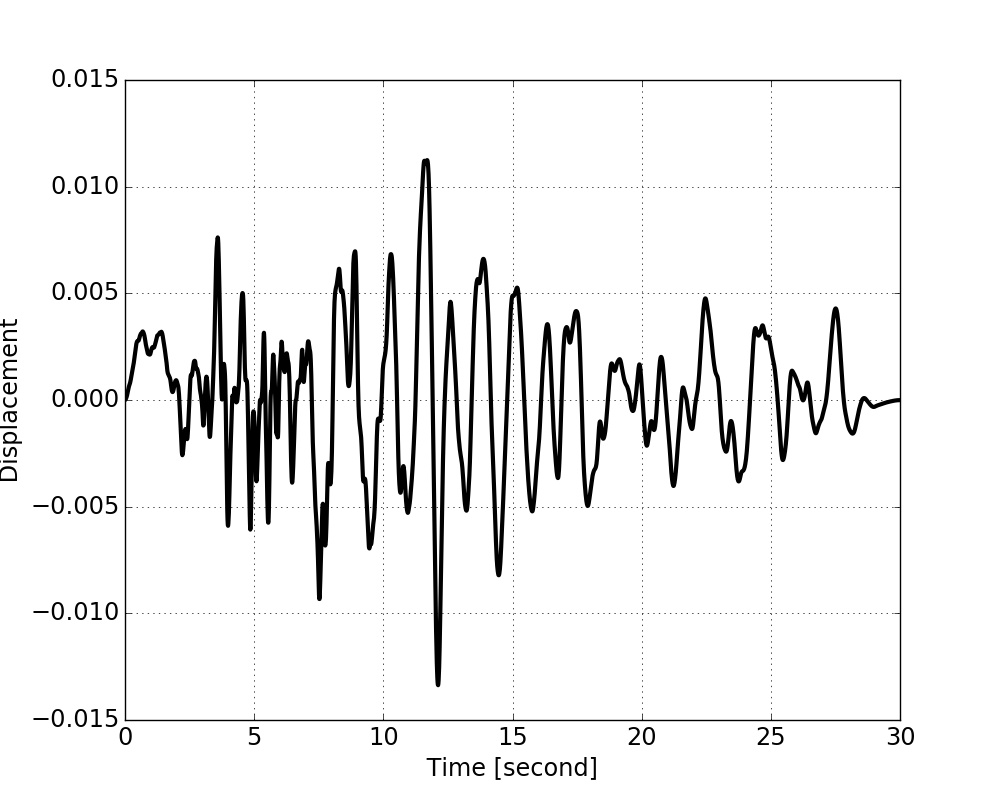
\includegraphics[width = 5cm]{./Figure-files/Day1/Nuclear_Power_Plant_with_3by1D_motions_from_Deconvolution/scaled_NORTHR_y_D.jpg}
  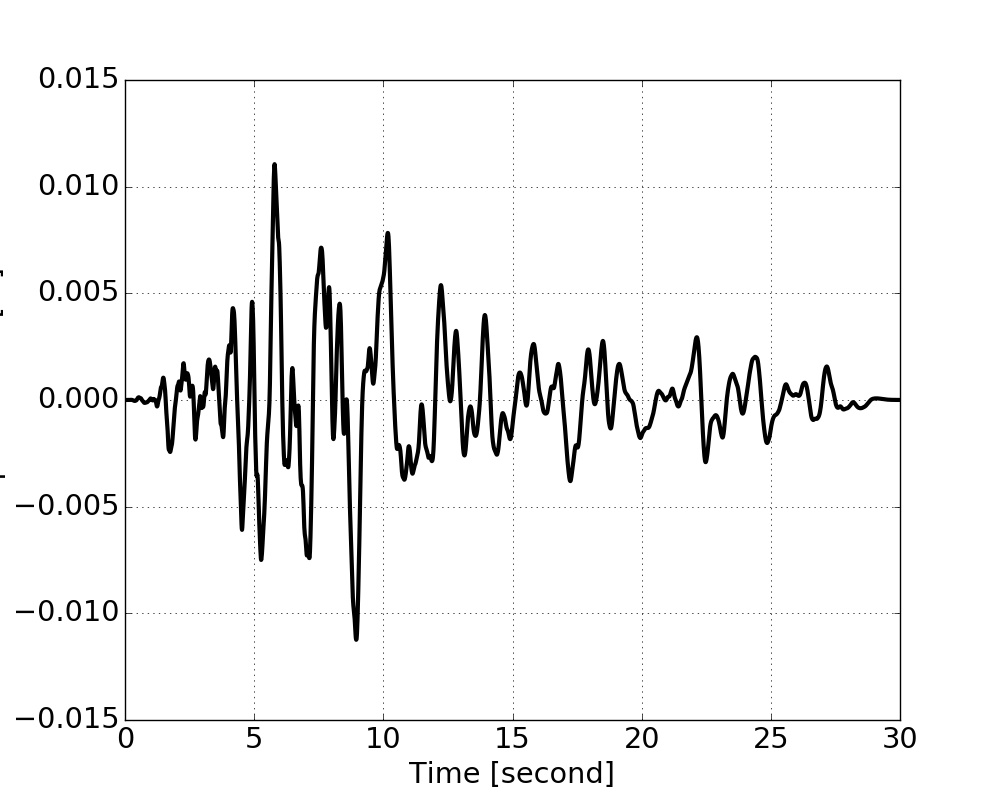
\includegraphics[width = 5cm]{./Figure-files/Day1/Nuclear_Power_Plant_with_3by1D_motions_from_Deconvolution/scaled_NORTHR_z_D.jpg}
  \caption{Displacement Deconvolution, from left to right in x, y, z directions respectively. }
  \label{fig_motion_deconvolution3}
\end{figure}


The Modeling parameters are listed.
\begin{itemize}
  \item Soil 
  \begin{itemize}
    \item Unit weight, $\gamma$, \enspace \enspace 21.4 kPa
    \item Shear velocity, $Vs$, \enspace \enspace 500 m/s
    \item Young's modulus, $E$, \enspace \enspace 1.3 GPa
    \item Poisson's ratio, $\nu$, \enspace \enspace 0.25
    \item Shear strength, $S_u$, \enspace \enspace 650 kPa
    \item von Mises radius, $k$, \enspace \enspace 60 kPa
    \item kinematic hardening, $H_a$, \enspace \enspace 30 MPa
    \item kinematic hardening, $C_r$, \enspace \enspace 25
  \end{itemize}
  \item Structure
  \begin{itemize}
    \item Unit weight, $\gamma$, \enspace \enspace 24 kPa
    \item Young's modulus, $E$, \enspace \enspace 20 GPa
    \item Poisson's ratio, $\nu$, \enspace \enspace 0.21
  \end{itemize}
\end{itemize}

% ******************************************************************
% ******************************************************************
% ******************************************************************
\clearpage
\newpage
\section{Single element Models: illustrate the elastic-plastic behavior}
\label{Single_element_Models_illustrate_the_elastic-plastic_behavior}

The compressed package of Real-ESSI input files for this example with von-Mises material model are available 
\href{https://github.com/yuan-energy/Real-ESSI-Short-Course-Examples/blob/master/short-course-examples/Day1/Single_element_Models_illustrate_the_elastic-plastic_behavior/vonMises/vonMises.tgz?raw=true}{HERE}. 

The compressed package of Real-ESSI input files for this example with Drucker-Prager material model are available 
\href{https://github.com/yuan-energy/Real-ESSI-Short-Course-Examples/blob/master/short-course-examples/Day1/Single_element_Models_illustrate_the_elastic-plastic_behavior/DruckerPrager/DruckerPrager.tgz?raw=true}{HERE}. 



The Modeling parameters are listed.
\begin{itemize}
  \item von-Mises linear hardening material model 
  \begin{itemize}
    \item Mass Density, $\rho$, \enspace \enspace 0.0 $kg/m^3$
    \item Young's modulus, $E$, \enspace \enspace 20 MPa
    \item Poisson's ratio, $\nu$, \enspace \enspace 0.0
    \item von Mises radius, $k$, \enspace \enspace 100 kPa
    \item kinematic hardening rate, $K_{kine} $, \enspace \enspace 2 MPa
    \item isotropic hardening rate, $K_{iso} $, \enspace \enspace 0 Pa
  \end{itemize}
  \item Drucker-Prager nonlinear hardening material model 
  \begin{itemize}
    \item Mass Density, $\rho$, \enspace \enspace 0.0 $kg/m^3$
    \item Young's modulus, $E$, \enspace \enspace 20 MPa
    \item Poisson's ratio, $\nu$, \enspace \enspace 0.0
    \item Drucker-Prager, $k$, \enspace \enspace 0.179527
    \item nonlinear kinematic hardening, $H_a$, \enspace \enspace 20 MPa
    \item nonlinear kinematic hardening, $C_r$, \enspace \enspace 100
    \item isotropic hardening rate, $K_{iso} $, \enspace \enspace 0 Pa
    \item initial confining stress, $p_0$, \enspace \enspace 1 Pa
  \end{itemize}
\end{itemize}


\begin{figure}[H]
  \centering
  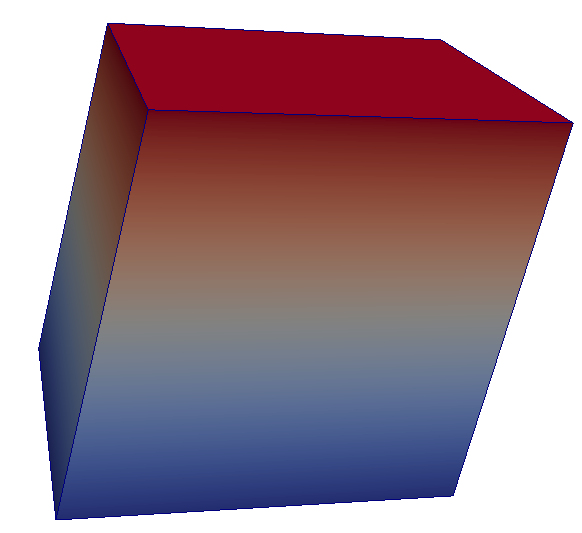
\includegraphics[width = 6cm]{./Figure-files/Day1/Single_element_Models_illustrate_the_elastic-plastic_behavior/overview.png}
  \caption{Simulation Model of Single Element}
  \label{fig_single_element_elastic-plastic}
\end{figure}

The illustrative nonlinear material behavior is shown in Fig.~\ref{fig_day1_illustration_nonlinear_single_element}.

\begin{figure}[H]
  \centering
  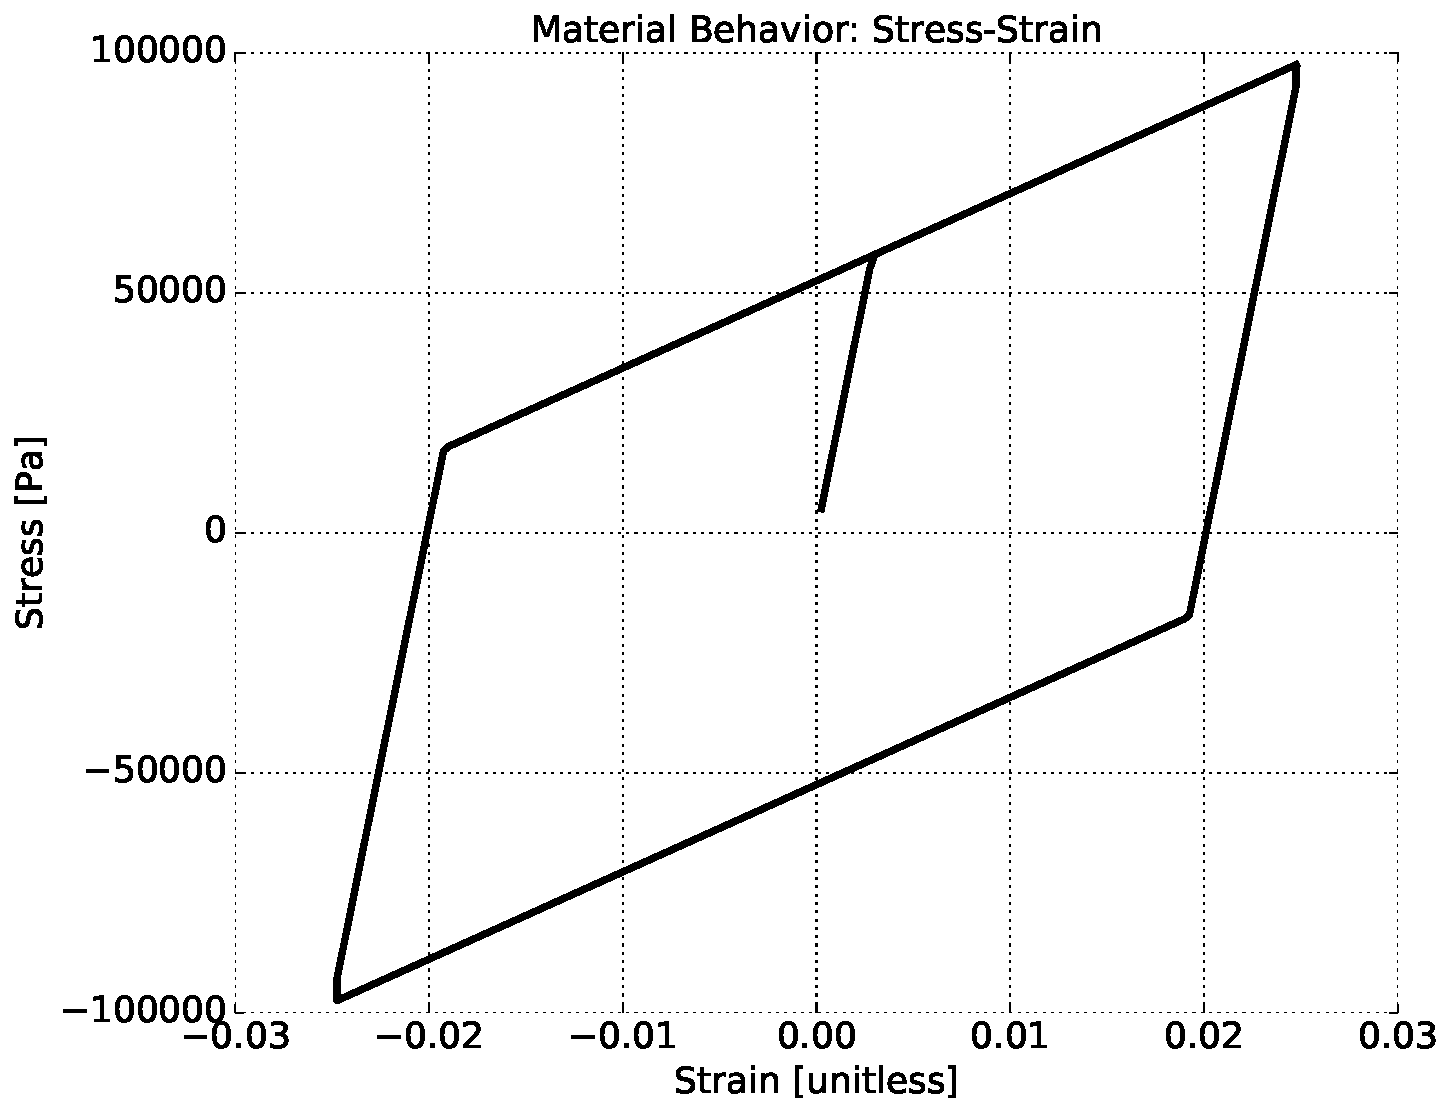
\includegraphics[width = 7cm]{./Figure-files/Day1/Single_element_Models_illustrate_the_elastic-plastic_behavior/vonMises.pdf}
  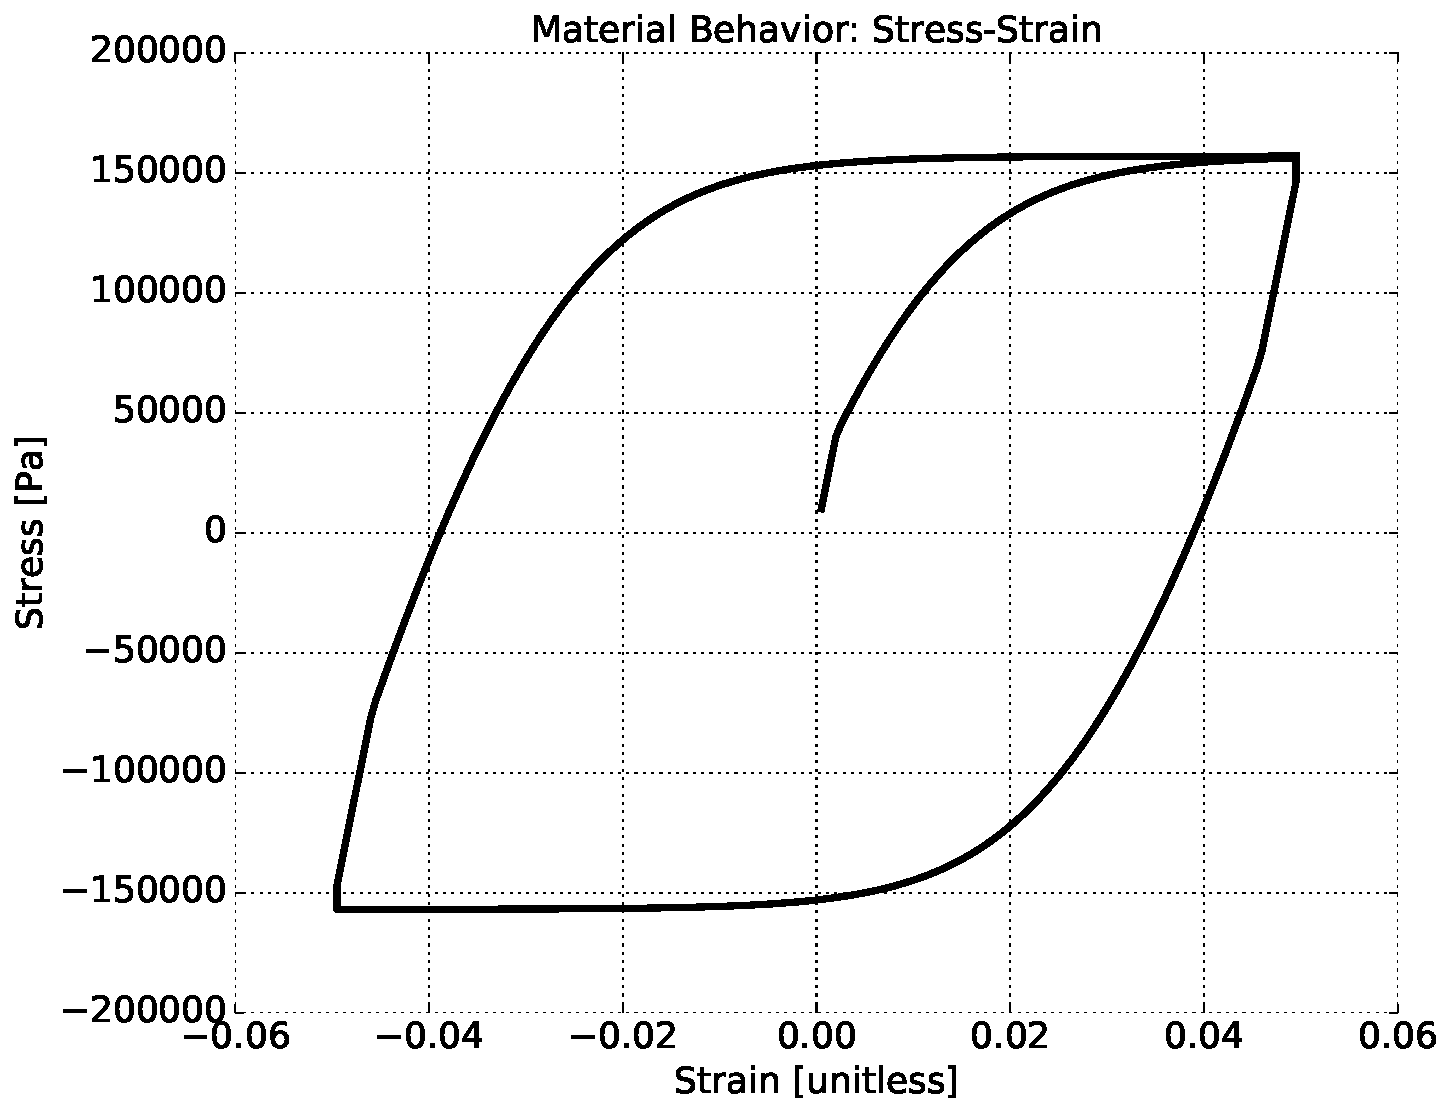
\includegraphics[width = 7cm]{./Figure-files/Day1/Single_element_Models_illustrate_the_elastic-plastic_behavior/DruckerPrager.pdf}
  \caption{ Illustration of Nonlinear Material Behavior }
  \label{fig_day1_illustration_nonlinear_single_element}
\end{figure}



% ******************************************************************
% ******************************************************************
% ******************************************************************
\clearpage
\newpage
\section{Pushover for Nonlinear Frame}
\label{Pushover_for_Nonlinear_Frame}


The Real-ESSI input files for this example are available 
\href{https://github.com/yuan-energy/Real-ESSI-Short-Course-Examples/tree/master/short-course-examples/Day1/Pushover_for_Nonlinear_Frame}{HERE}. 
The compressed package of Real-ESSI input files for this example is available 
\href{https://github.com/yuan-energy/Real-ESSI-Short-Course-Examples/blob/master/short-course-examples/Day1/Pushover_for_Nonlinear_Frame/Pushover_for_Nonlinear_Frame.tgz?raw=true}{HERE}. 

\begin{figure}[H]
  \centering
  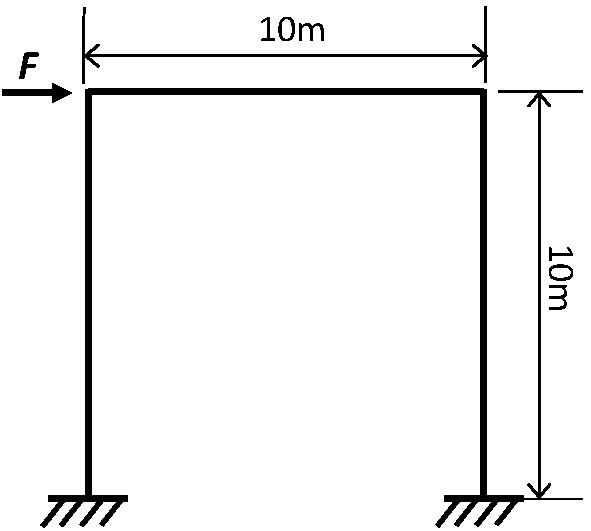
\includegraphics[width = 6cm]{./Figure-files/Day1/Pushover_for_Nonlinear_Frame/overview.pdf}
  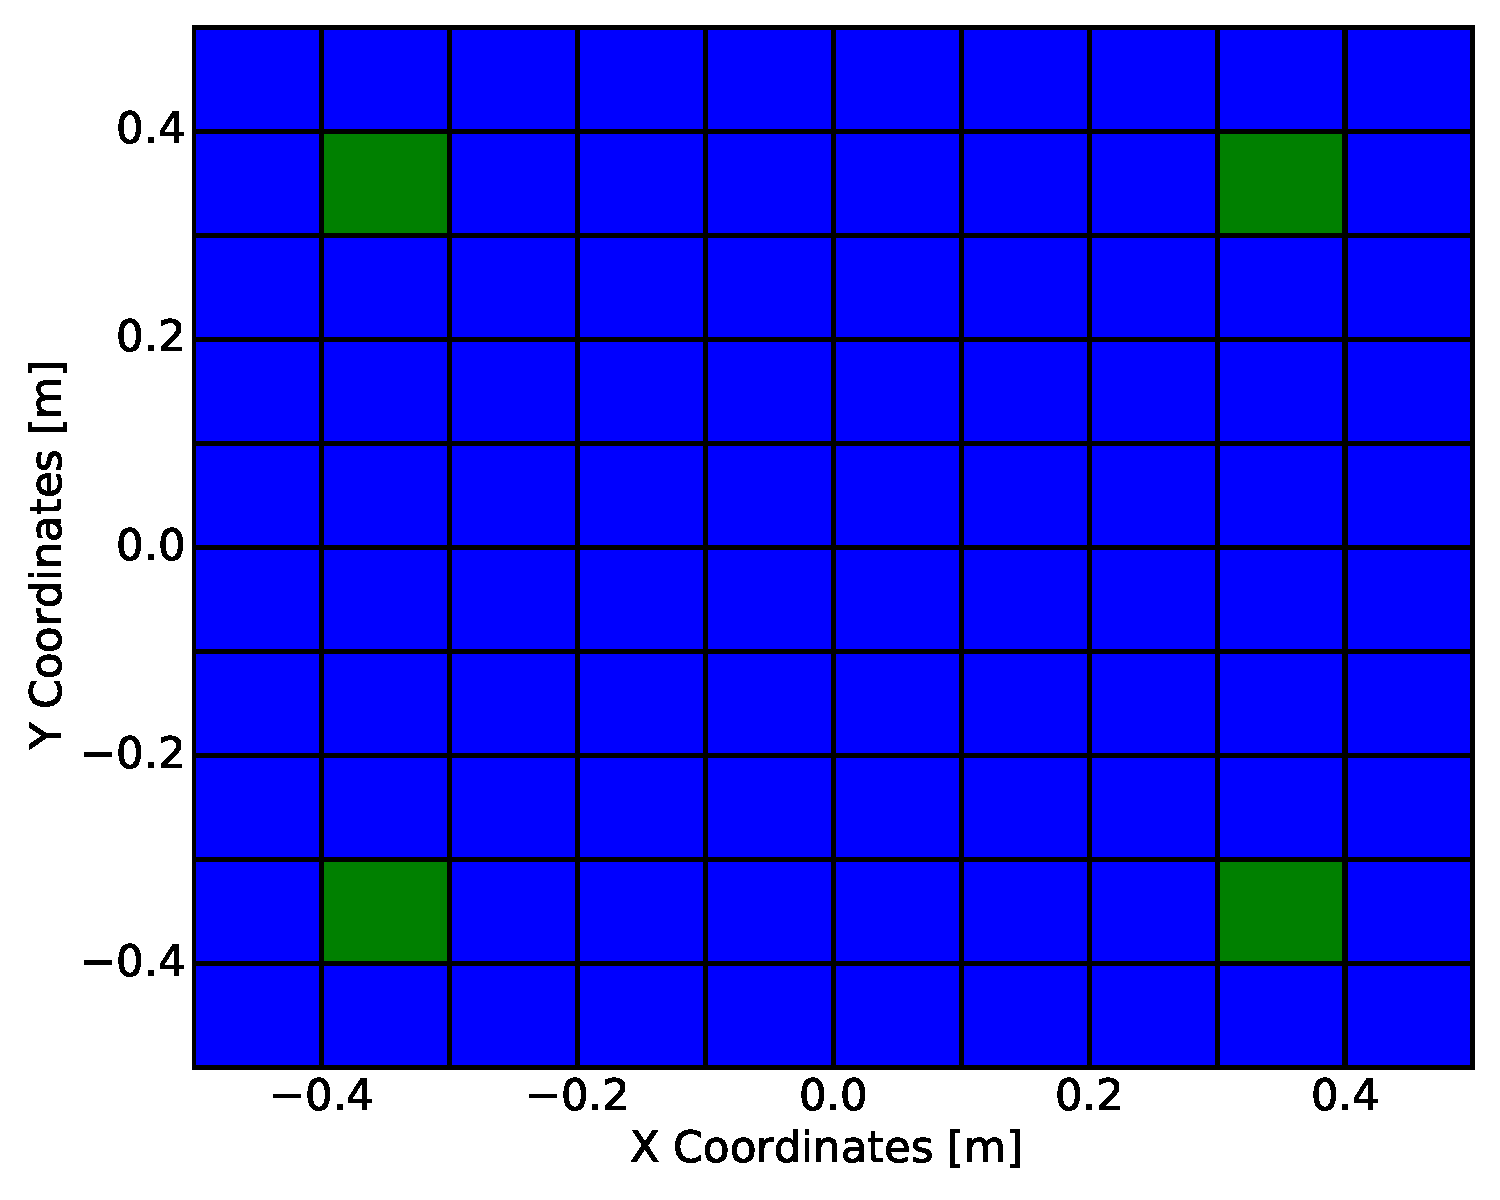
\includegraphics[width = 6cm]{./Figure-files/Day1/Pushover_for_Nonlinear_Frame/rectangle_rebar2.pdf}
  \caption{Model of Pushover Simulation and the Cross Section of Fiber Beam (Concrete and Rebar) }
  \label{fig_single_element_pushover}
\end{figure}

The illustrative result is shown in Fig.~\ref{fig_day1_fiberbeam_pushover_results}.
\begin{figure}[H]
  \centering
  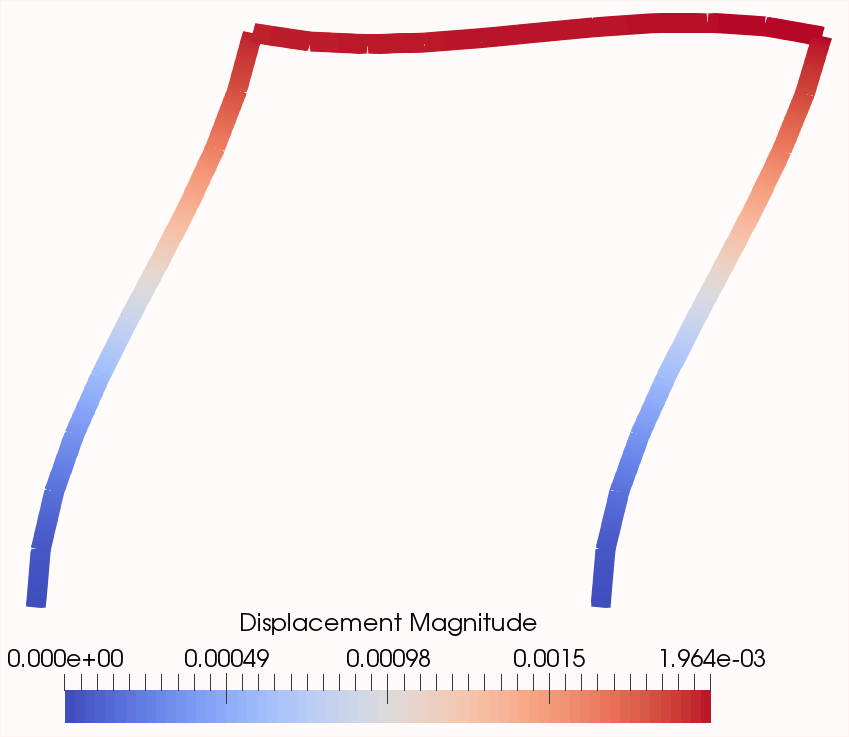
\includegraphics[width = 8cm]{./Figure-files/Day1/Pushover_for_Nonlinear_Frame/fiberBeamDeform.png}
  \caption{Illustration results of Fiber Pushover}
  \label{fig_day1_fiberbeam_pushover_results}
\end{figure}


The Modeling parameters are listed.
\begin{itemize}
  \item Uniaxial concrete 
  \begin{itemize}
    \item Compressive strength,  \enspace \enspace 24 MPa
    \item Strain at compressive strength,  \enspace \enspace 0.001752
    \item Crushing strength,  \enspace \enspace 0.0 Pa
    \item Strain at compressive strength,  \enspace \enspace 0.003168
    \item lambda, \enspace \enspace 0.5
    \item Tensile strength, \enspace \enspace 0 Pa
    \item Tension softening stiffness, \enspace \enspace 0 Pa
  \end{itemize}
  \item Uniaxial steel
  \begin{itemize}
    \item Yield strength, \enspace \enspace 413.8 MPa
    \item Young's modulus, \enspace \enspace 200 GPa
    \item Strain hardening ratio, \enspace \enspace 0.01
    \item R0, \enspace \enspace 18.0
    \item cR1,  \enspace \enspace 0.925
    \item cR2,  \enspace \enspace 0.15
    \item a1, \enspace \enspace 0.0
    \item a2, \enspace \enspace 55.0
    \item a3, \enspace \enspace 0.0
    \item a4, \enspace \enspace 55.0
  \end{itemize}
\end{itemize}


% ******************************************************************
% ******************************************************************
% ******************************************************************
\clearpage
\newpage
\section{Preprocess examples with Gmsh}
\label{Preprocess_examples_with_Gmsh}
\subsection{Cantilever Example}


The Real-ESSI input files for this example are available 
\href{https://github.com/yuan-energy/Real-ESSI-Short-Course-Examples/blob/master/short-course-examples/Day1/Preprocess_examples_with_Gmsh/cantilever}{HERE}. 
The compressed package of Real-ESSI input files for this example is available 
\href{https://github.com/yuan-energy/Real-ESSI-Short-Course-Examples/blob/master/short-course-examples/Day1/Preprocess_examples_with_Gmsh/cantilever/cantilever.tgz?raw=true}{HERE}. 


\begin{figure}[H]
  \centering
  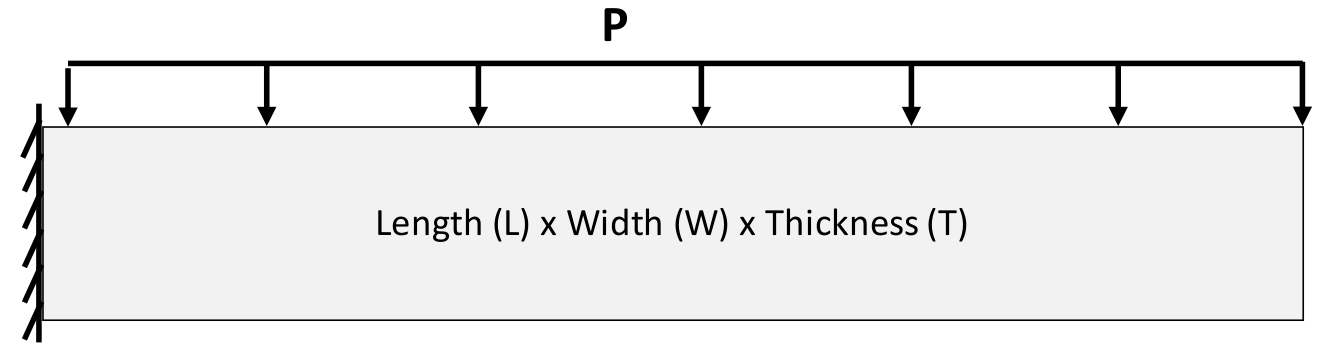
\includegraphics[width = 10cm]{./Figure-files/Day1/Preprocess_examples_with_Gmsh/example1/overview.png}
  \caption{Simulation Model Cantilever}
  \label{fig_gmsh_ex1}
\end{figure}


The illustration results is shown in Fig.~\ref{fig_day1_gmsh_ex_cantilever_results}.

\begin{figure}[H]
  \centering
  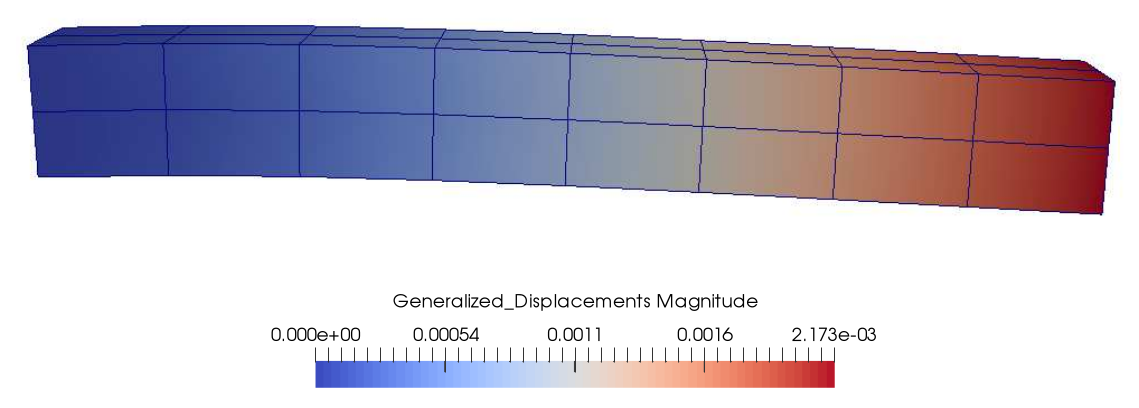
\includegraphics[width = 10cm]{./Figure-files/Day1/Preprocess_examples_with_Gmsh/example1/cantilever_results.png}
  \caption{Simulation Model Cantilever Illustration Results }
  \label{fig_day1_gmsh_ex_cantilever_results}
\end{figure}




% ******************************************************************
% ******************************************************************
\clearpage
\newpage
\subsection{Brick-shell-beam Example}

The Real-ESSI input files for this example are available 
\href{https://github.com/yuan-energy/Real-ESSI-Short-Course-Examples/blob/master/short-course-examples/Day1/Preprocess_examples_with_Gmsh/brick-shell-beam}{HERE}. 
The compressed package of Real-ESSI input files for this example is available 
\href{https://github.com/yuan-energy/Real-ESSI-Short-Course-Examples/blob/master/short-course-examples/Day1/Preprocess_examples_with_Gmsh/brick-shell-beam/brick-shell-beam.tgz?raw=true}{HERE}. 



\begin{figure}[H]
  \centering
  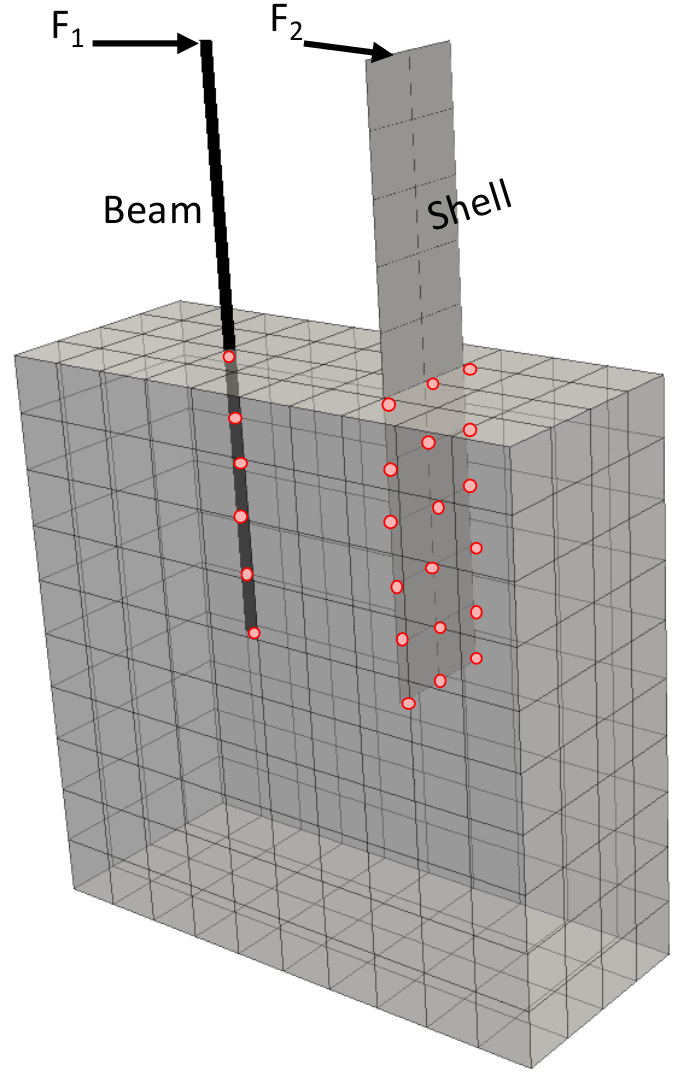
\includegraphics[width = 5cm]{./Figure-files/Day1/Preprocess_examples_with_Gmsh/example2/overview.png}
  \caption{Simulation Model Brick-Shell-Beam}
  \label{fig_gmsh_ex2}
\end{figure}


The illustration results is shown in Fig.~\ref{fig_day1_gmsh_ex_beam_shell_brick}.

\begin{figure}[H]
  \centering
  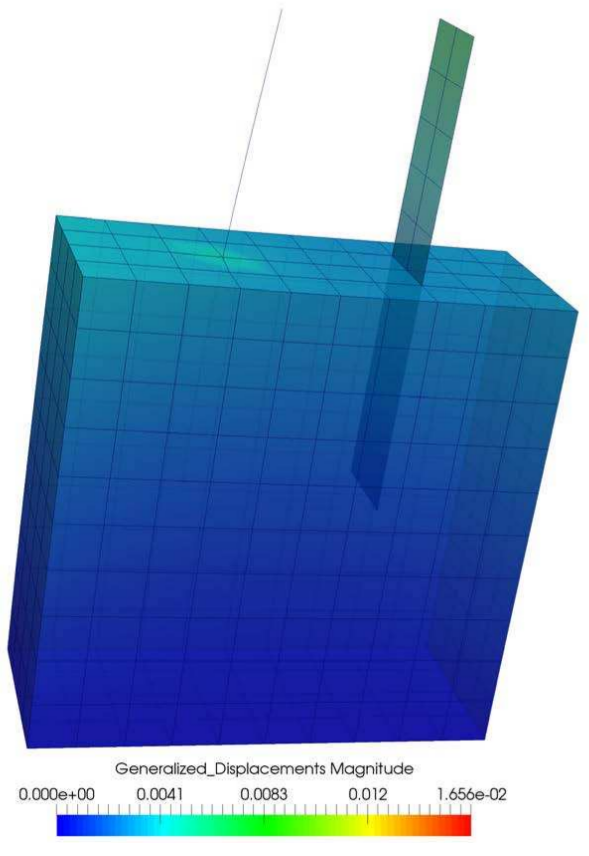
\includegraphics[width = 6cm]{./Figure-files/Day1/Preprocess_examples_with_Gmsh/example2/beam-shell-results-visual.png}
  \caption{Brick-Shell-Beam Illustration Results }
  \label{fig_day1_gmsh_ex_beam_shell_brick}
\end{figure}


% ******************************************************************
% ******************************************************************
\clearpage
\newpage
\subsection{DRM 2D Example}

The Real-ESSI input files for this example are available 
\href{https://github.com/yuan-energy/Real-ESSI-Short-Course-Examples/blob/master/short-course-examples/Day1/Preprocess_examples_with_Gmsh/DRM2D}{HERE}. 
The compressed package of Real-ESSI input files for this example is available 
\href{https://github.com/yuan-energy/Real-ESSI-Short-Course-Examples/blob/master/short-course-examples/Day1/Preprocess_examples_with_Gmsh/DRM2D/DRM2D.tgz?raw=true}{HERE}. 

\begin{figure}[H]
  \centering
  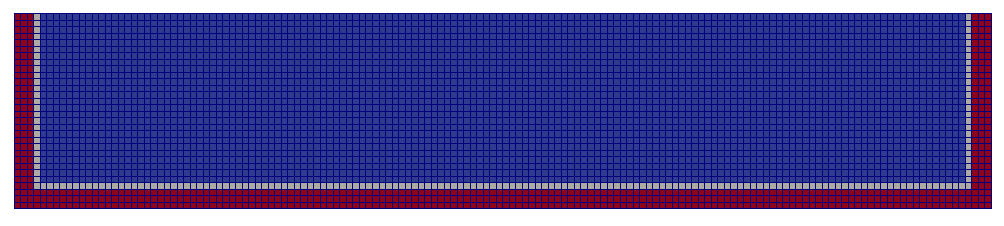
\includegraphics[width = 10cm]{./Figure-files/Day1/Preprocess_examples_with_Gmsh/example3/overview.png}
  \caption{Simulation Model DRM 2D}
  \label{fig_gmsh_ex3}
\end{figure}

The illustration results of free field DRM 2D Model under 1D motion is shown 
in Fig.~\ref{fig_day1_DRM2D_results}. 

\begin{figure}[H]
  \centering
  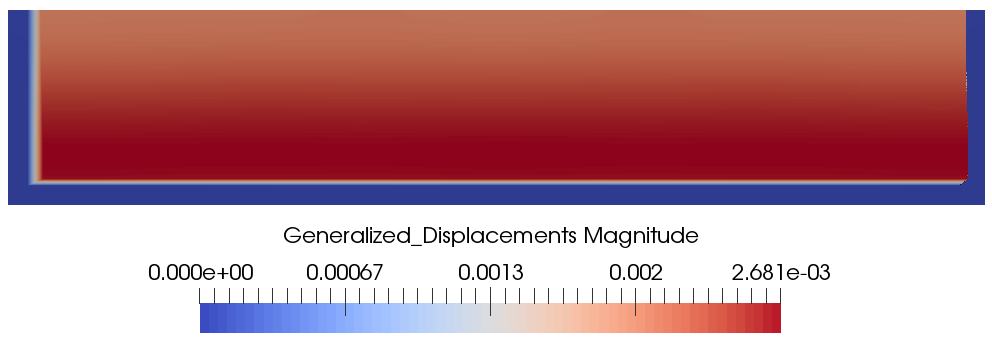
\includegraphics[width = 10cm]{./Figure-files/Day1/Preprocess_examples_with_Gmsh/example3/DRM2D_results.png}
  \caption{Simulation Model DRM 2D}
  \label{fig_day1_DRM2D_results}
\end{figure}

% ******************************************************************
% ******************************************************************
\clearpage
\newpage
\subsection{DRM 3D Example}


The Real-ESSI input files for this example are available 
\href{https://github.com/yuan-energy/Real-ESSI-Short-Course-Examples/blob/master/short-course-examples/Day1/Preprocess_examples_with_Gmsh/DRM3D}{HERE}. 
The compressed package of Real-ESSI input files for this example is available 
\href{https://github.com/yuan-energy/Real-ESSI-Short-Course-Examples/blob/master/short-course-examples/Day1/Preprocess_examples_with_Gmsh/DRM3D/DRM3D.tgz?raw=true}{HERE}. 

\begin{figure}[H]
  \centering
  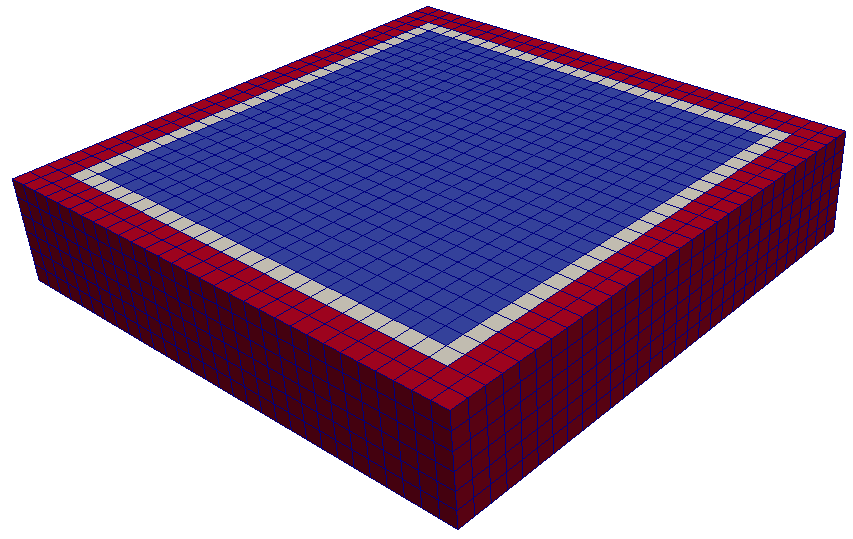
\includegraphics[width = 10cm]{./Figure-files/Day1/Preprocess_examples_with_Gmsh/example4/overview.png}
  \caption{Simulation Model DRM 3D}
  \label{fig_gmsh_ex4}
\end{figure}

The illustration results of free field DRM 3D Model under 1D motion is shown 
in Fig.~\ref{fig_day1_DRM3D_results}. 

\begin{figure}[H]
  \centering
  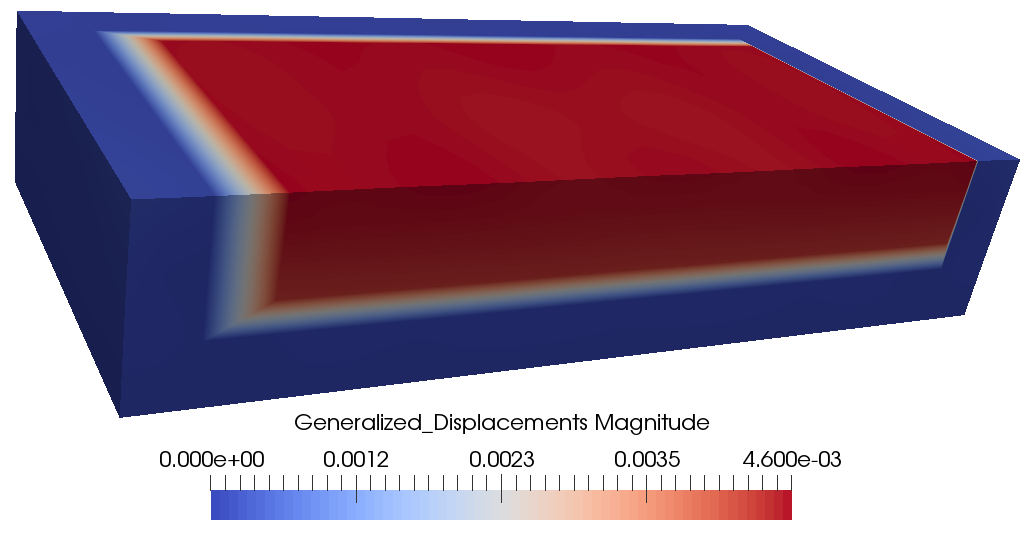
\includegraphics[width = 10cm]{./Figure-files/Day1/Preprocess_examples_with_Gmsh/example4/DRM3D_results.png}
  \caption{Simulation Model DRM 2D}
  \label{fig_day1_DRM3D_results}
\end{figure}


% ******************************************************************
% ******************************************************************
% ******************************************************************
\clearpage
\newpage
\section{Postprocess examples with Paraview}
\label{Postprocess_examples_with_Paraview}
\subsection{Slice Visualization}

The Real-ESSI input files for this example are available 
\href{https://github.com/yuan-energy/Real-ESSI-Short-Course-Examples/tree/master/short-course-examples/Day1/Nuclear_Power_Plant_with_1D_motions_from_Deconvolution}{HERE}. 
The compressed package of Real-ESSI input files for this example is available 
\href{https://github.com/yuan-energy/Real-ESSI-Short-Course-Examples/blob/master/short-course-examples/Day1/Nuclear_Power_Plant_with_1D_motions_from_Deconvolution/Nuclear_Power_Plant_with_1D_motions_from_Deconvolution.tgz?raw=true}{HERE}.  

\begin{figure}[H]
  \centering
  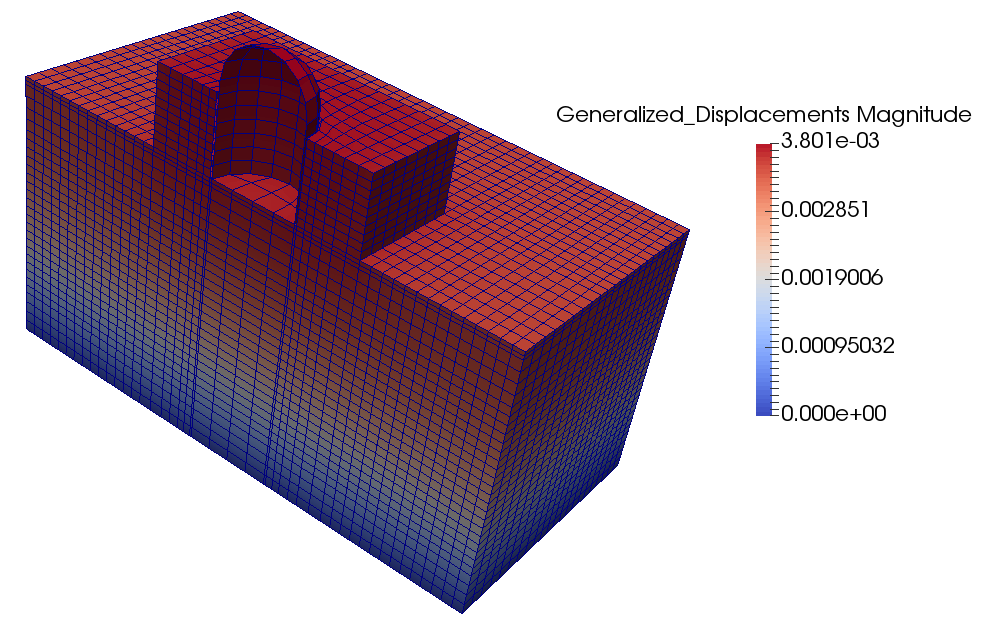
\includegraphics[width = 10cm]{./Figure-files/Day1/Postprocess_examples_with_Paraview/slide_visualization.png}
  \caption{Slice Visualization with Paraview}
  \label{fig_paraview_slice}
\end{figure}


% ******************************************************************
% ******************************************************************
\clearpage
\newpage
\subsection{Stress Visualization}

The Real-ESSI input files for this example are available 
\href{https://github.com/yuan-energy/Real-ESSI-Short-Course-Examples/tree/master/short-course-examples/Day1/Nuclear_Power_Plant_with_1D_motions_from_Deconvolution}{HERE}. 
The compressed package of Real-ESSI input files for this example is available 
\href{https://github.com/yuan-energy/Real-ESSI-Short-Course-Examples/blob/master/short-course-examples/Day1/Nuclear_Power_Plant_with_1D_motions_from_Deconvolution/Nuclear_Power_Plant_with_1D_motions_from_Deconvolution.tgz?raw=true}{HERE}.  

\begin{figure}[H]
  \centering
  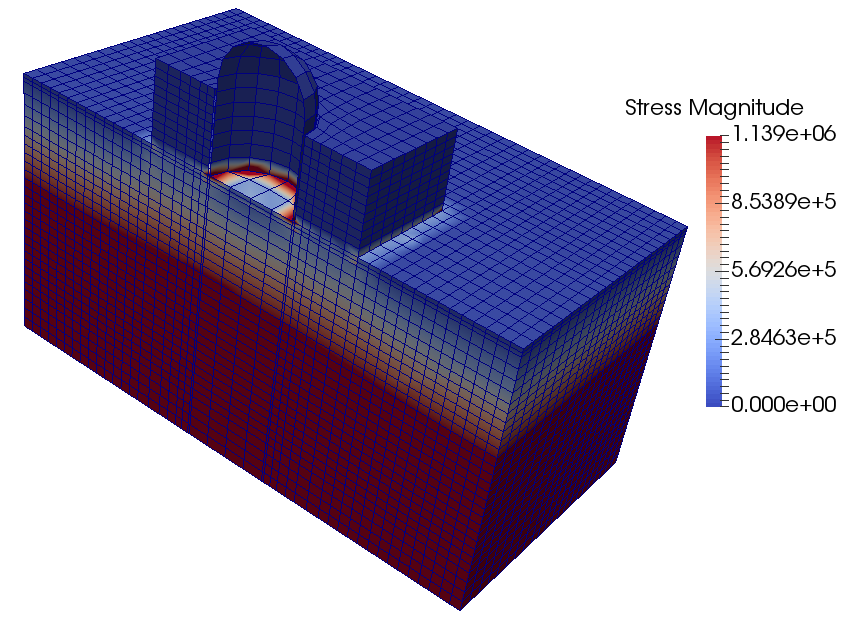
\includegraphics[width = 10cm]{./Figure-files/Day1/Postprocess_examples_with_Paraview/stress_visualization.png}
  \caption{Stress Visualization with Paraview}
  \label{fig_paraview_stress}
\end{figure}

% % ******************************************************************
% % ******************************************************************
% \clearpage
% \newpage
% \subsection{Pore Pressure Visualization in upU Element}

% The Real-ESSI input files for this example are available 
% \href{https://github.com/yuan-energy/Real-ESSI-Short-Course-Examples/tree/master/short-course-examples/Day1/Postprocess_examples_with_Paraview/upU}{HERE}. 
% The compressed package of Real-ESSI input files for this example is available 
% \href{https://github.com/yuan-energy/Real-ESSI-Short-Course-Examples/blob/master/short-course-examples/Day1/Postprocess_examples_with_Paraview/upU/upU.tgz?raw=true}{HERE}.  

% \begin{figure}[H]
%   \centering
%   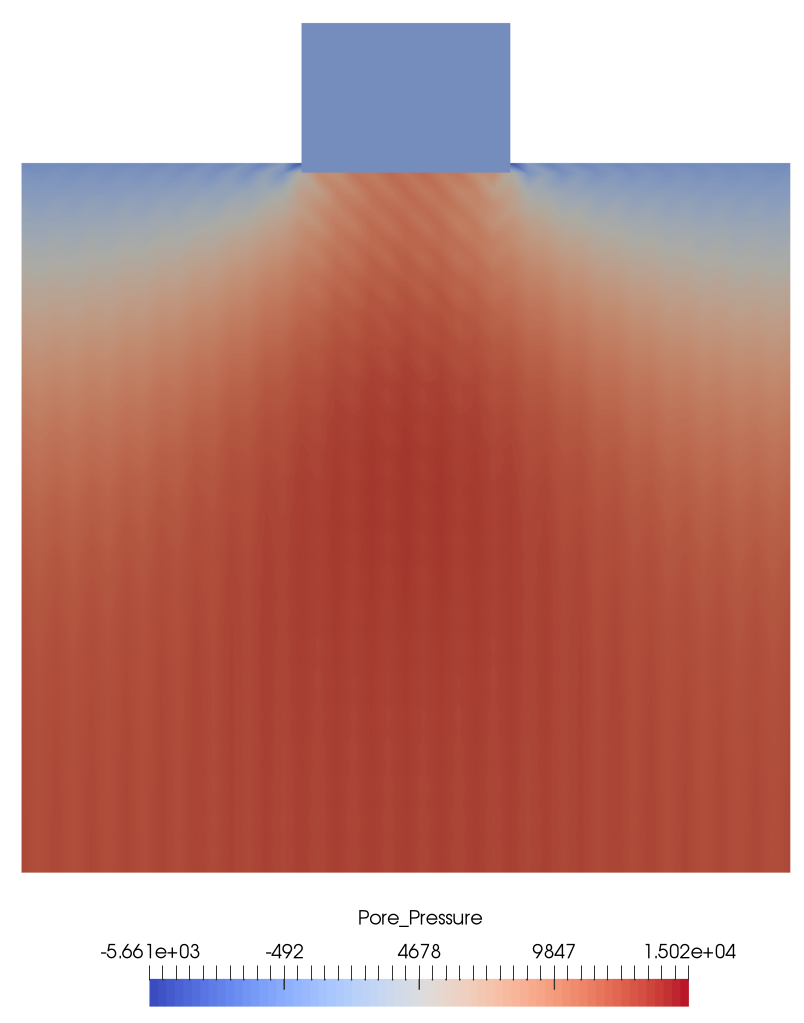
\includegraphics[width = 8cm]{./Figure-files/Day1/Postprocess_examples_with_Paraview/pore_pressure.png}
%   \caption{Pore Pressure Visualization with Paraview}
%   \label{fig_paraview_pore_pressure}
% \end{figure}



% ******************************************************************
% ******************************************************************
\clearpage
\newpage
\subsection{Eigen Visualization}


The Real-ESSI input files for this example are available 
\href{https://github.com/yuan-energy/Real-ESSI-Short-Course-Examples/tree/master/short-course-examples/Day1/Postprocess_examples_with_Paraview/eigen}{HERE}. 
The compressed package of Real-ESSI input files for this example is available 
\href{https://github.com/yuan-energy/Real-ESSI-Short-Course-Examples/blob/master/short-course-examples/Day1/Postprocess_examples_with_Paraview/eigen/eigen.tgz?raw=true}{HERE}.  

\begin{figure}[H]
  \centering
  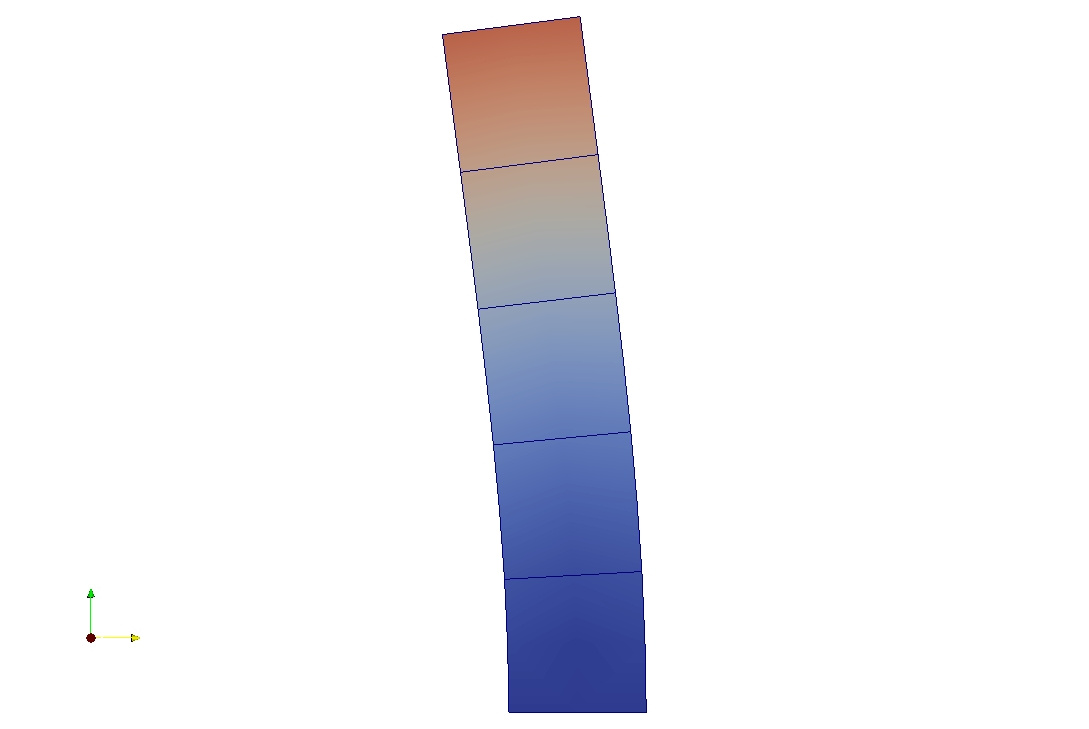
\includegraphics[width = 8cm]{./Figure-files/Day1/Postprocess_examples_with_Paraview/eigenmode1.jpg}
  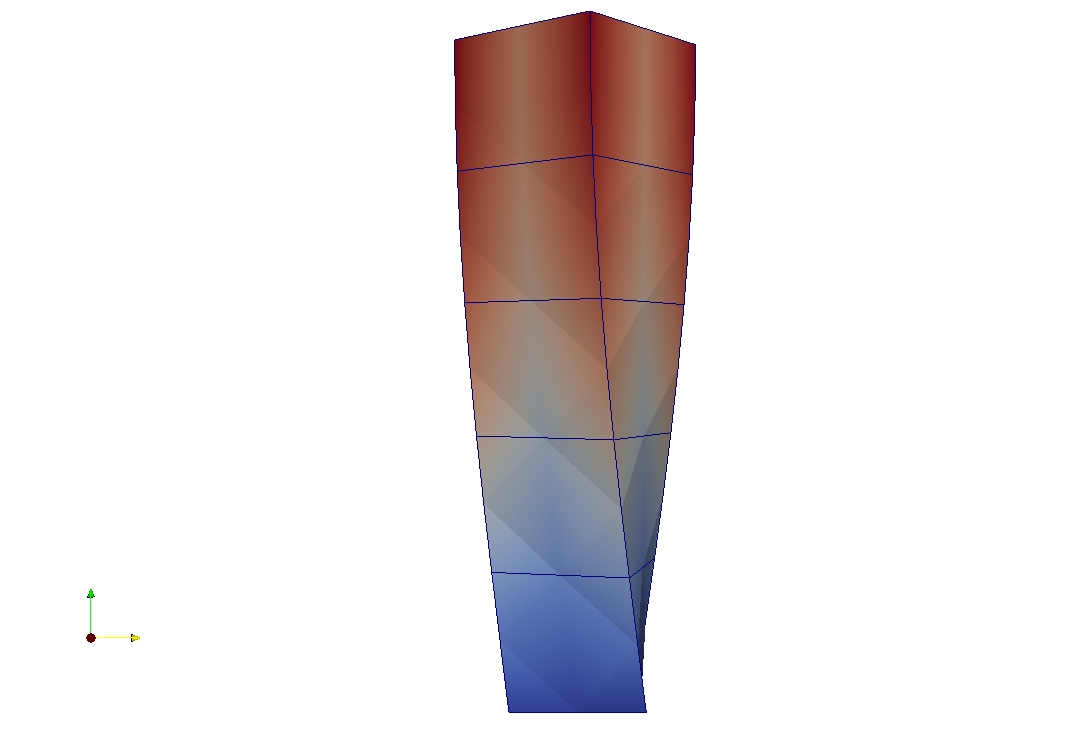
\includegraphics[width = 8cm]{./Figure-files/Day1/Postprocess_examples_with_Paraview/eigenmode2.jpg}
  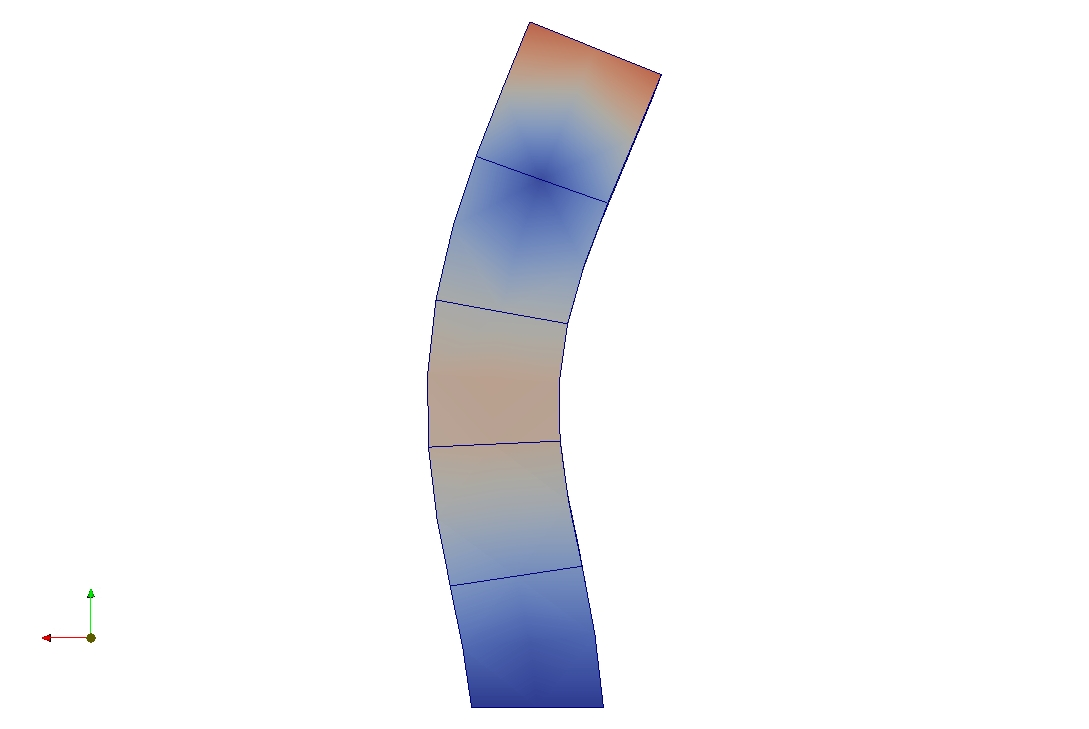
\includegraphics[width = 8cm]{./Figure-files/Day1/Postprocess_examples_with_Paraview/eigenmode3.jpg}
  \caption{Eigen Mode Visualization with Paraview}
  \label{fig_paraview_eigen}
\end{figure}


% ******************************************************************
% ******************************************************************
% ******************************************************************
\clearpage
\newpage
\section{Check Model and Visualization of Boundary Conditions}
\label{Check_Model_and_Visualization_of_Boundary_Conditions}

The Real-ESSI input files for this example are available 
\href{https://github.com/yuan-energy/Real-ESSI-Short-Course-Examples/tree/master/short-course-examples/Day1/Check_Model_and_Visualization_of_Boundary_Conditions}{HERE}. 
The compressed package of Real-ESSI input files for this example is available 
\href{https://github.com/yuan-energy/Real-ESSI-Short-Course-Examples/blob/master/short-course-examples/Day1/Check_Model_and_Visualization_of_Boundary_Conditions/Check_Model_and_Visualization_of_Boundary_Conditions.tgz?raw=true}{HERE}. 

\begin{figure}[H]
  \centering
  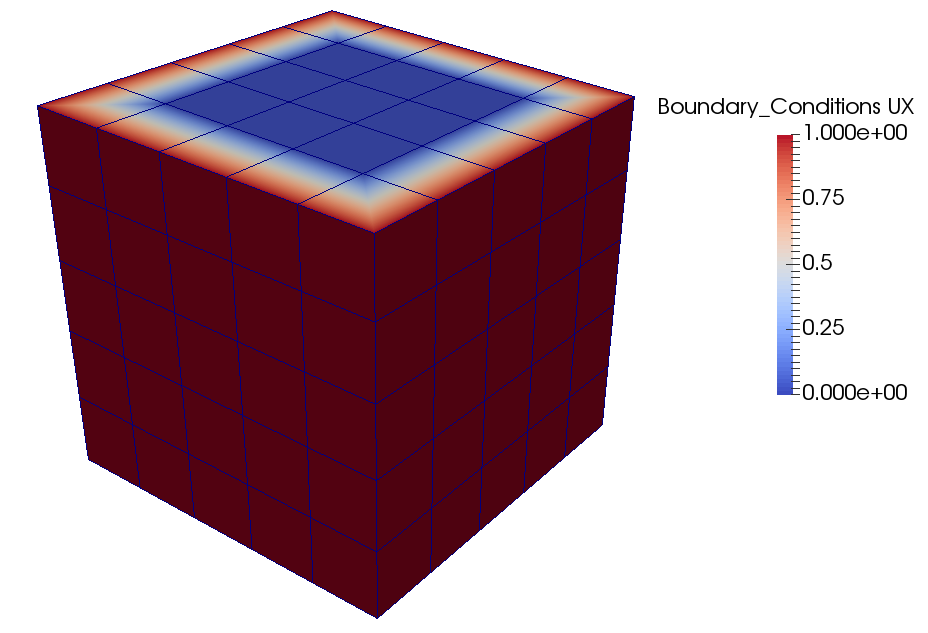
\includegraphics[width = 10cm]{./Figure-files/Day1/Check_Model_and_Visualization_of_Boundary_Conditions/boundary_ux.png}
  \caption{Partition Information Visualization with Paraview}
  \label{fig_check_model_and_boundary_condition_ux}
\end{figure}



\begin{figure}[H]
  \centering
  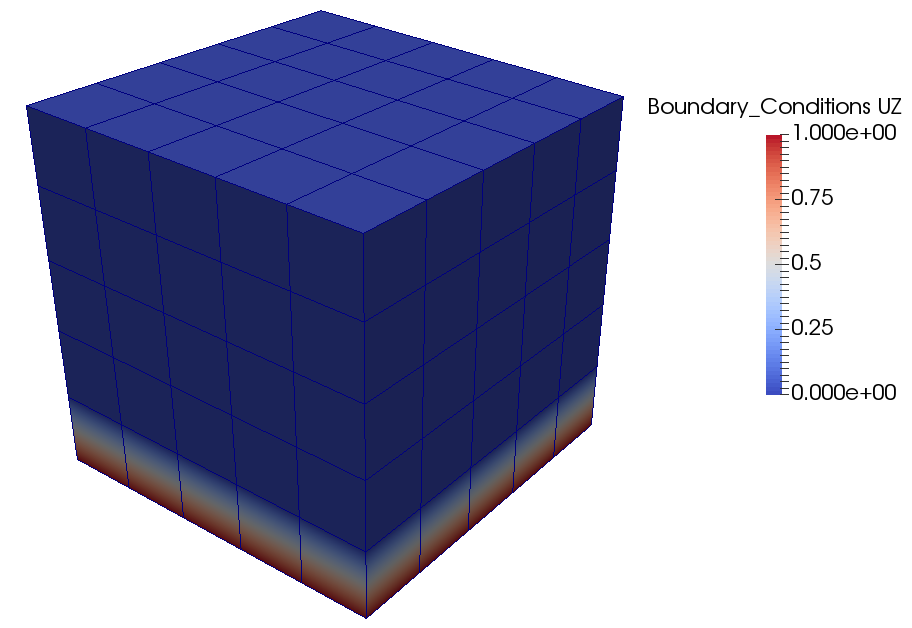
\includegraphics[width = 10cm]{./Figure-files/Day1/Check_Model_and_Visualization_of_Boundary_Conditions/boundary_uz.png}
  \caption{Partition Information Visualization with Paraview}
  \label{fig_check_model_and_boundary_condition_uz}
\end{figure}




% ******************************************************************
% ******************************************************************
% ******************************************************************
\clearpage
\newpage
\section{Restart Simulation}
\label{Restart_Simulation}

\subsection{ Restart in the next stage }

The Real-ESSI input files for this example are available 
\href{https://github.com/yuan-energy/Real-ESSI-Short-Course-Examples/tree/master/short-course-examples/Day1/Restart_Simulation/between_stages}{HERE}. 
The compressed package of Real-ESSI input files for this example is available 
\href{https://github.com/yuan-energy/Real-ESSI-Short-Course-Examples/blob/master/short-course-examples/Day1/Restart_Simulation/between_stages/between_stages.tgz?raw=true}{HERE}. 

\begin{figure}[H]
  \centering
  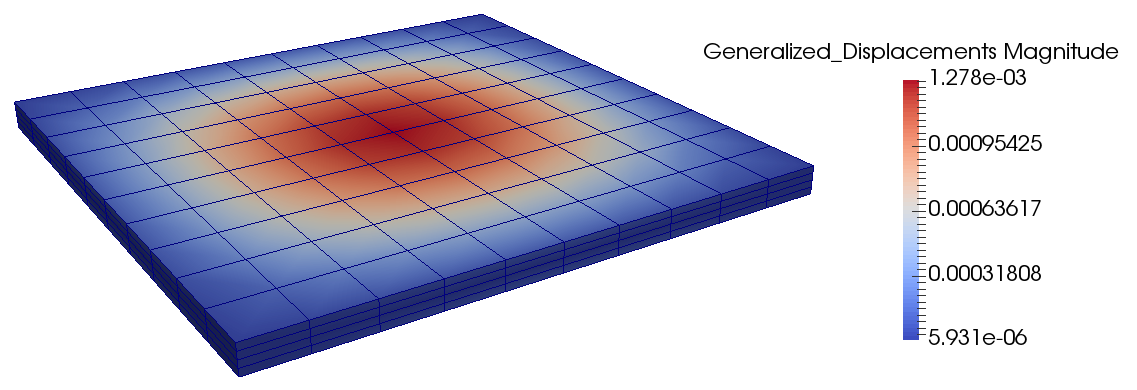
\includegraphics[width = 10cm]{./Figure-files/Day1/Restart_Simulation/restart.png}
  \caption{Restart Simulation}
  \label{fig_restart_simulation1}
\end{figure}

This group of examples illustrate the restart functionality between loading stages. 
There are three test cases in this example.
The two loading stages in the first test case is splitted into two test cases to show the restart feature.
\begin{itemize}
  \item The first test case run through two loading stages.
  \item The second test case only run the first loading stage and saves model state at the end.
  \item The third test case restart the simulation from the saved model state of the second test case. 
      Then, with the restarted model state, the test cases run the second loading stage only. 
\end{itemize}

Finally, the results of the third test case are exactly the same to the first test case.



% ******************************************************************
% ******************************************************************
\clearpage
\newpage
\subsection{ Restart inside the stage }
For the case of inconvergence, restart with the previous loading stage.

The Real-ESSI input files for this example are available 
\href{https://github.com/yuan-energy/Real-ESSI-Short-Course-Examples/tree/master/short-course-examples/Day1/Restart_Simulation/in_stage}{HERE}. 
The compressed package of Real-ESSI input files for this example is available 
\href{https://github.com/yuan-energy/Real-ESSI-Short-Course-Examples/blob/master/short-course-examples/Day1/Restart_Simulation/in_stage/in_stage.tgz?raw=true}{HERE}. 

\begin{figure}[H]
  \centering
  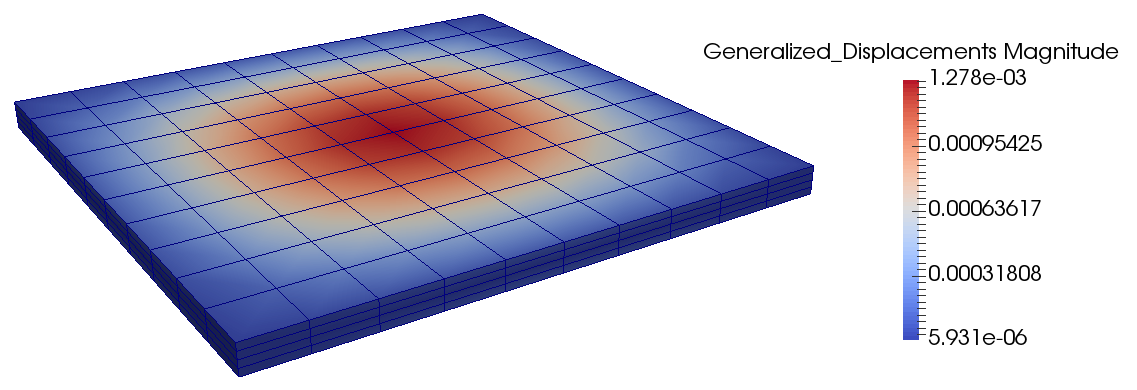
\includegraphics[width = 10cm]{./Figure-files/Day1/Restart_Simulation/restart.png}
  \caption{Restart Simulation}
  \label{fig_restart_simulation2}
\end{figure}


This group of examples illustrate the restart functionality inside one loading stage 
when the simulation cannot converge in the nonlinear analysis.
The nonlinear material model, von-Mises Armstrong-Frederick, is used in all test cases.

There are three test cases in this example.
\begin{itemize}
  \item The first test case run through the whole simulation with a relatively big tolerance of the unbalanced force.
  \item The second test case failed in the middle of the simulation with a relatively small tolerance of the unbalanced force.
      When the second test failed, the model reverted to the last commit model state and saved model state.
  \item The third test case load the saved model state, increased the tolerance of the unbalanced force, and added the 
      remaining load to the model to continue the simulation.
\end{itemize}

Finally, the results of the third test case are exactly the same to the first test case.

Note that in the third test case only the remaining load should be added to the model. 
Whenever the new loading stage is used, the previous loading are all finished,
which means that the static loading becomes constant and the dynamic loading vanishes.





